\documentclass[conference]{IEEEtran}
\IEEEoverridecommandlockouts
% The preceding line is only needed to identify funding in the first footnote. If that is unneeded, please comment it out.
\usepackage{cite}
\usepackage{amsmath,amssymb,amsfonts}
\usepackage{algorithmic}
\usepackage{graphicx}
\usepackage{textcomp}
\usepackage{xcolor}
\usepackage[utf8]{inputenc}
\usepackage[T1]{fontenc}
\usepackage{polski}
\usepackage{babel}

\def\BibTeX{{\rm B\kern-.05em{\sc i\kern-.025em b}\kern-.08em
    T\kern-.1667em\lower.7ex\hbox{E}\kern-.125emX}}

\begin{document}

\title{Projekt Zespołowy: Zaawansowane Metody Uczenia Maszynowego\\
}

\author{
\IEEEauthorblockN{Alicja Osam-Gyaabin }
\and
\IEEEauthorblockN{Mikołaj Zawada}
\and
\IEEEauthorblockN{Karol Kociołek}
}

\maketitle

\begin{abstract}
Celem projektu jest opracowanie dwóch modeli uczenia przez wzmacnianie w wybranym środowisku. W ramach projektu przeprowadzono analizę środowiska Tennis, opisano dwa różne algorytmy RL oraz wytrenowano modele, które zostały porównane.
\end{abstract}


\end{IEEEkeywords}


\section{Wybór i Opis Środowiska}
\subsection{Wybór Środowiska} Do realizacji projektu zdecydowano się na wykorzystanie środowiska \textit{Tennis}, będącego częścią rodziny środowisk Atari dostępnych w bibliotece Gymnasium.  Szczegółowa dokumentacja dostępna jest pod adresem: \url{https://www.gymlibrary.dev/environments/atari/tennis/}.

\begin{figure}[htbp] \centering 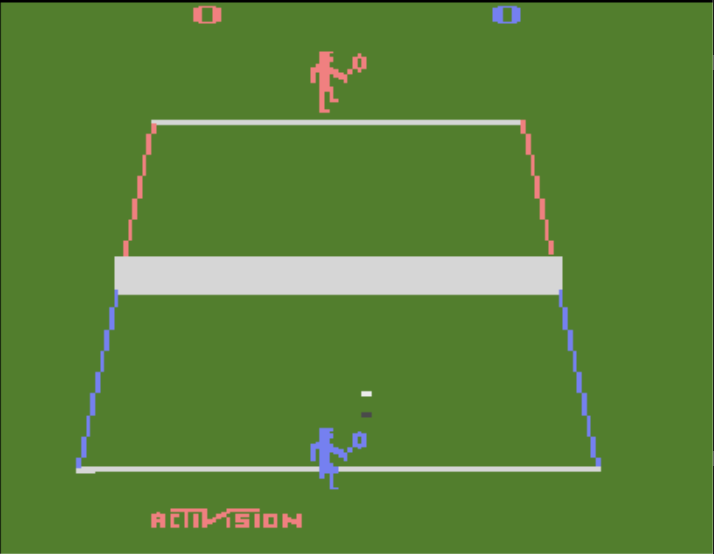
\includegraphics[width=0.45\textwidth]{image1.png} \caption{Przykładowy obraz ze środowiska \textit{Tennis}} \label{fig:tennis} \end{figure}

\subsection{Opis Środowiska}
Środowisko Tennis symuluje mecz tenisa, w którym użytkownik kontroluje pomarańczowego zawodnika rywalizującego z komputerowo sterowanym niebieskim przeciwnikiem. Rozgrywka odbywa się zgodnie z zasadami tenisa, gdzie zwycięzcą zostaje ten zawodnik, który pierwszy zdobędzie co najmniej sześć gemów z przewagą minimum dwóch gemów. W przypadku osiągnięcia remisu 6-6, mecz kontynuowany jest aż jeden z zawodników zdobędzie przewagę dwóch gemów.

\subsubsection{Przestrzeń Akcji}
Przestrzeń akcji w środowisku \textit{Tennis} jest dyskretna i obejmuje 18 możliwych działań, które agent może podjąć w trakcie gry. Akcje te pozwalają na realizację podstawowych ruchów, takich jak poruszanie się w górę, w dół, w lewo i w prawo, a także   uderzenia piłki w różnych kierunkach i serwy.


\subsubsection{Przestrzeń Obserwacji}

Przestrzeń obserwacji w środowisku \textit{Tennis} jest reprezentowana przez obraz w formacie RGB o wymiarach 210 pikseli wysokości, 160 pikseli szerokości i 3 kanałach kolorów (odpowiadających czerwieni, zieleni i niebieskiemu). Obraz dostarcza agentowi szczegółowych informacji o stanie środowiska, takich jak pozycje zawodników, trajektoria piłki, linie kortu czy siatka.




\subsubsection{Importowanie Środowiska} Aby zaimportować środowisko \textit{Tennis} w języku Python, można skorzystać z poniższego fragmentu kodu: \begin{verbatim} env = gym.make("ALE/Tennis-v5") \end{verbatim}


\section{Wybór i Opis Algorytmów}
Wybrano dwa algorytmy RL:

\subsection{Proximal Policy Optimization (PPO)}

Proximal Policy Optimization (PPO) to algorytm uczenia ze wzmocnieniem, który optymalizuje politykę tak, aby maksymalizować oczekiwany zwrot (\textit{reward}), ograniczając jednocześnie zbyt duże zmiany w polityce.

Poniżej przedstawiono kluczowe elementy algorytmu PPO:
\begin{itemize}
    \item \textit{Polityka:} Polityka $\pi_\theta(a|s)$ określa prawdopodobieństwo wykonania akcji $a$ w stanie $s$. Parametry $\theta$ są trenowane przy użyciu sieci neuronowej.
    \item \textit{Funkcja korzyści:} Funkcja korzyści $A(s, a)$ mierzy, jak dobra była dana akcja $a$ w stanie $s$ w porównaniu do oczekiwań.
    \item \textit{Ograniczenie zmian w polityce:} PPO wprowadza funkcję celu z ograniczeniem (\textit{clipped objective}), która ogranicza zbyt duże zmiany w polityce, aby zapewnić stabilność uczenia.
\end{itemize}

\subsubsection{Funkcja celu PPO}
Funkcja celu PPO opiera się na współczynniku prawdopodobieństwa:
\[
r_t(\theta) = \frac{\pi_\theta(a_t|s_t)}{\pi_{\theta_{\text{old}}}(a_t|s_t)},
\]
gdzie $\pi_\theta$ to nowa polityka, a $\pi_{\theta_{\text{old}}}$ to polityka sprzed aktualizacji.

Celem PPO jest maksymalizacja następującej funkcji:
\[
L^{\text{CLIP}}(\theta) = \mathbb{E}_t \left[ \min\left( r_t(\theta)A_t, \text{clip}(r_t(\theta), 1 - \epsilon, 1 + \epsilon)A_t \right) \right],
\]
gdzie:
\begin{itemize}
    \item $r_t(\theta)$ to stosunek nowych do starych prawdopodobieństw,
    \item $A_t$ to funkcja korzyści, która uwzględnia różnicę między oczekiwaniami a rzeczywistym wynikiem,
    \item $\epsilon$ to hiperparametr, który określa dopuszczalny zakres zmian (zazwyczaj $\epsilon = 0.1$ lub $\epsilon = 0.2$),
    \item $\text{clip}(r_t(\theta), 1 - \epsilon, 1 + \epsilon)$ ogranicza wartość współczynnika, aby zmiany w polityce były umiarkowane.
\end{itemize}

\subsubsection{Główne kroki algorytmu PPO}
Algorytm PPO składa się z następujących etapów:
\begin{enumerate}
    \item Generowanie trajektorii: Symulator zbiera dane (stany, akcje, nagrody) w oparciu o bieżącą politykę $\pi_\theta$.
    \item Obliczanie funkcji korzyści: Na podstawie zebranych danych obliczana jest funkcja korzyści $A_t$, np. przy użyciu metody Generalized Advantage Estimation (GAE).
    \item Aktualizacja polityki: Maksymalizowana jest funkcja celu $L^{\text{CLIP}}(\theta)$ przy użyciu algorytmu gradientowego.
    \item Aktualizacja funkcji wartości: Model uczy się funkcji wartości $V(s)$, która przewiduje oczekiwaną nagrodę w danym stanie.
    \item Powtarzanie procesu: Po aktualizacji modelu zbierane są nowe dane i proces jest kontynuowany.
\end{enumerate}

PPO jest skutecznym i stosunkowo prostym algorytmem, który znajduje zastosowanie w różnych dziedzinach, takich jak gry komputerowe.





\section{Trenowanie Modeli RL}

\subsection{Model 1: Proximal Policy Optimization (PPO)}
\begin{figure}[htbp] \centering 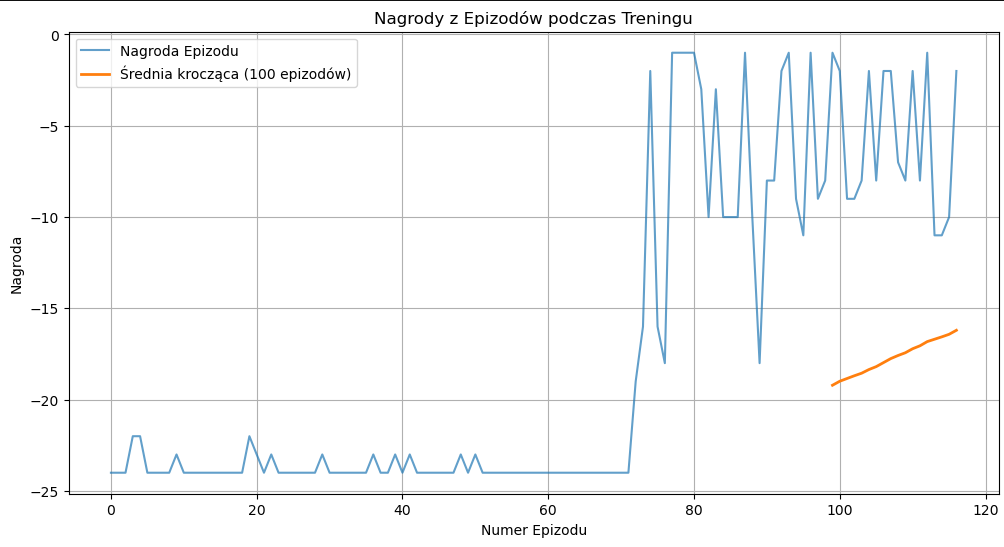
\includegraphics[width=0.45\textwidth]{image.png} \caption{Trening PPO \textit{Tennis}} \label{fig:tennis} \end{figure}





\section{Wnioski}




\end{document}